\documentclass[12pt]{article}
\usepackage{amsmath}
\usepackage{geometry}
\usepackage{graphicx}
\usepackage{hyperref}
\usepackage[latin1]{inputenc}
\usepackage{listings}
\usepackage[dvipsnames]{xcolor}
\renewcommand{\labelitemi}{$\textendash$}
\geometry{
    a4paper,
    total={170mm,257mm},
    left=20mm,
    right=20mm,
    top=15mm,
    bottom=15mm
}

\title{CS7DS2: Week 4 Assignment}
\author{Conor McCauley - 17323203}
\date{March 1, 2022}

\begin{document}

\maketitle

\section*{Functions}

The two functions that will be used during this assignment are:

$$f_1(x, y) = 9 (x - 5)^4 + 10 (y - 2)^2$$
$$f_2(x, y) = \max(x - 5, 0) + 10 \cdot |y - 2|$$

Using SymPy we can initialise two symbols, $x$ and $y$, and define both functions using those symbols (SymPy's built-in \texttt{Abs()} and \texttt{Max()} functions are used when defining $f_2$). Using the \texttt{diff()} function we can differentiate both functions with respect to both $x$ and $y$ resulting in the following:

$$\frac{\partial f_1}{\partial x} = 36 (x - 5)^3,\, \frac{\partial f_1}{\partial y} = 20y - 40$$
$$\frac{\partial f_2}{\partial x} = \theta(x - 5),\, \frac{\partial f_2}{\partial y} = 10\cdot sign(y - 2)$$

\section*{Question (a)}

In the code snippets provided for each of the gradient descent functions all references to \texttt{x} indicate an array of parameters, eg $[x, y]$, and all references to \texttt{df} indicate an array of lambda functions calculating the partial derivatives of the primary function, eg $[\frac{\partial f_1}{\partial x}, \frac{\partial f_1}{\partial y}]$. The variable \texttt{n} indicates the number of parameters, eg $f_1(x, y)$ has two parameters.

\subsection*{(i) Polyak Step Size}

At each iteration a constant step size is calculated by taking the value of the function for the given parameter values and dividing it by the sum of the squares of the gradients (the partial derivatives) for each parameter. To prevent division by zero a very small $\epsilon$ is added to the denominator. Technically, before the value of the function is divided by the sum of square gradients it is decremented by $f^*$ which, in our case, we just set to zero and therefore ignore. Each parameter is then decremented by the product of the calculated step size and the parameter's gradient.

\lstset{basicstyle=\footnotesize}
\begin{lstlisting}[language=Python]
# each iteration:
step = f(*x) / (sum(df[i](x[i]) ** 2 for i in range(n)) + epsilon)
for i in range(n):
    x[i] -= step * df[i](x[i])
\end{lstlisting}

\subsection*{(ii) RMSProp}

Prior to running any iterations two empty arrays are initialised containing the step sizes and sums of historical square gradients for each parameter, respectively. The step sizes are initially set to the value of the $\alpha_0$ parameter. At each iteration the parameter values are first decremented by the product of the initial step size and the parameter's gradient. The historical sum of square gradients is then updated by adding the current square of the parameter's gradient to the sum - the $\beta$ parameter controls how the current and historical gradients are weighted. The step sizes are then updated by dividing the constant $\alpha_0$ value by the square root of the current square gradient sum. As in (i), an $\epsilon$ is added to the denominator.

\lstset{basicstyle=\footnotesize}
\begin{lstlisting}[language=Python]
alphas = [alpha0] * n
sums = [0] * n
# each iteration:
for i in range(n):
    x[i] -= alphas[i] * df[i](x[i])
    sums[i] = (beta * sums[i]) + ((1 - beta) * (df[i](x[i]) ** 2))
    alphas[i] = alpha0 / ((sums[i] ** 0.5) + epsilon)
\end{lstlisting}

\subsection*{(iii) Heavy Ball}

Prior to running any iterations the value of $z$, a historical sum of square gradients, is set to zero. At each iteration, like in (ii), the historical sum of square gradients is updated with the $\beta$ parameter controlling the weight of the historical sum and the $\alpha$ parameter controlling the weight of the current sum. However, only a single step size is used (as opposed to one for each parameter) and the sum of square gradients includes every parameter. As in (i), this sum divides the value of the function for the given parameter values minus $f^*=0$. Each parameter is then decremented by the product of the new step size, $z$, and its gradient.

\lstset{basicstyle=\footnotesize}
\begin{lstlisting}[language=Python]
z = 0
# each iteration:
z = (beta * z) + (alpha * f(*x) / (sum(df[i](x[i]) ** 2 for i in range(n)) + epsilon))
for i in range(n):
    x[i] -= z * df[i](x[i])
\end{lstlisting}

\subsection*{(iv) Adam}

Prior to running any iterations two empty arrays are initialised containing the weighted historical sums of both gradients and square gradients for each parameter, respectively. An iteration counter, $t$, is also set to zero. At each iteration the counter, $t$, is incremented by one. Then, for each parameter, almost exactly like in (ii), the historical sums of both regular gradients and square gradients are updated with the parameter $\beta_1$ controlling the weight of the regular gradients and the parameter $\beta_2$ controlling the weight of the square gradients. The new sums are then scaled by dividing them by one minus their weighting parameters to the power of the iteration counter $t$, eg $1 - \beta_1^t$. Finally, each parameter is decremented by the product of the $\alpha$ learning rate parameter and the scaled regular gradient sum divided by the square root of the scaled square gradient sum. An $\epsilon$ is added to the denominator once again.

\lstset{basicstyle=\footnotesize}
\begin{lstlisting}[language=Python]
ms = [0] * n
vs = [0] * n
t = 0
# each iteration:
t += 1
for i in range(n):
    ms[i] = (beta1 * ms[i]) + ((1 - beta1) * df[i](x[i]))
    vs[i] = (beta2 * vs[i]) + ((1 - beta2) * (df[i](x[i]) ** 2))
    m_hat = ms[i] / (1 - (beta1 ** t))
    v_hat = vs[i] / (1 - (beta2 ** t))
    x[i] -= alpha * (m_hat / ((v_hat ** 0.5) + epsilon))
\end{lstlisting}

\section*{Question (b)}

\subsection*{(i) RMSProp}

Parameter values of $\alpha_0 \in \{0.001, 0.01, 0.1\}$ and $\beta \in \{0.25, 0.9\}$ where investigated with $x_0 = 3, y_0 = 0$ and 200 iterations of the algorithm being run.

For $f_1$ in both cases where $\alpha_0=0.1$ the algorithm greatly diverged to the point that its results are not visible on the plot below. When $\alpha_0=0.001$ the convergence rate of the algorithm is far too slow and it doesn't come close to reaching the minimum after 200 iterations. The optimal learning rate in this case appears to be $\alpha_0=0.01$ which converges after about 150 iterations. The value of $\beta$ does not appear to have much of an impact on the rate of convergence in these examples.

\begin{center}
    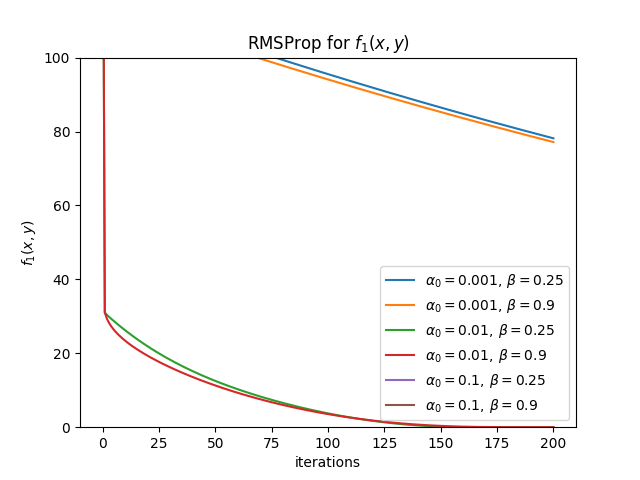
\includegraphics[scale=0.6]{figs/b/b_i_1.png}
\end{center}

For $f_2$ in cases where $\alpha_0=0.001$ the function decreases far too slowly to converge after a reasonable number of iterations. In both cases where $\alpha_0=0.1$ the function converges very quickly towards the minimum but begins to oscillate around a point slightly above the minimum indefinitely which leads to poor results. When $\alpha_0=0.01$ both examples do converge on values fairly close to the minimum (0.01 and 0.08) after around 180 iterations however they do not appear to decrease any further than this.

\begin{center}
    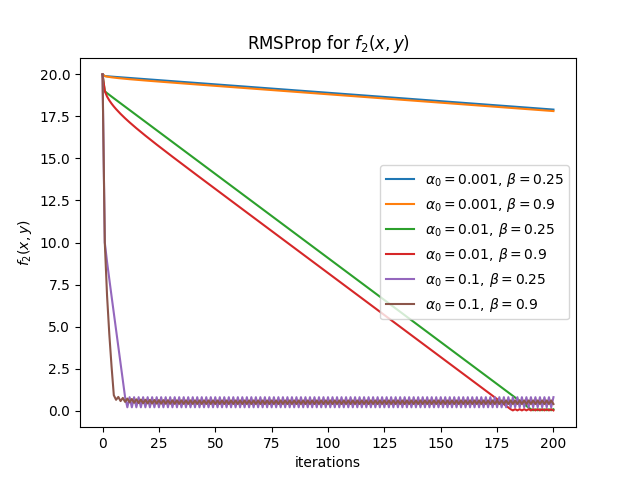
\includegraphics[scale=0.6]{figs/b/b_i_2.png}
\end{center}

For both functions the parameters of $\alpha_0=0.01$ and $\beta=0.9$ produced the best results.

\subsection*{(ii) Heavy Ball}

Parameter values of $\alpha \in \{0.01, 0.1, 1\}$ and $\beta \in \{0.25, 0.9\}$ where investigated with $x_0 = 3, y_0 = 0$ and 200 iterations of the algorithm being run.

For $f_1$ when $\alpha=0.01$ and $\beta=0.25$ the function converges too slowly and does not reach the minimum. When $\alpha=0.01$ but $\beta=0.9$ it does converge on the minimum after about 80 iterations. In both cases where $\alpha=0.1$ the function converges on the minimum fairly quickly although in the case where $\beta=0.9$ the function diverges wildly for a number of iterations before quickly returning to the minimum. When $\alpha=1$ both cases converge on the minimum rapidly but in the case of $\beta=0.9$ the function wildly diverges from the minimum it reached and never converges again.

\begin{center}
    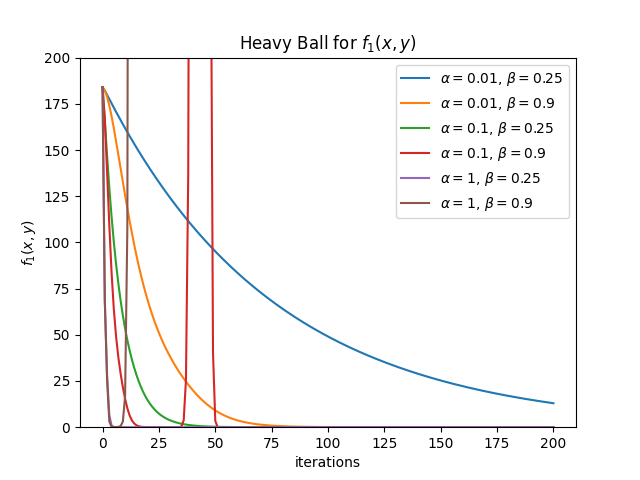
\includegraphics[scale=0.6]{figs/b/b_ii_1.png}
\end{center}

For $f_2$, like for $f_1$, when $\alpha=0.01$ and $\beta=0.25$ the function converges too slowly and does not reach the minimum and when $\beta=0.9$ it does converge on the minimum after about 30 iterations. When $\alpha=0.1$ and $\beta=0.25$ the function also converges on the minimum after about 30 iterations. When $\beta=0.9$ the function takes almost 100 iterations to converge due to the value oscillating up and down but still decreasing nonetheless. As was the case for $f_1$, when $\alpha=1$ and $\beta=0.9$ the function diverges rapidly but when $\beta=0.25$ the function converges on the minimum almost immediately.

\begin{center}
    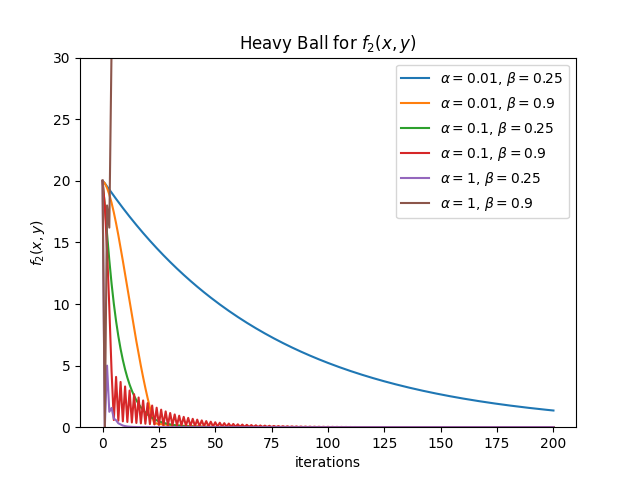
\includegraphics[scale=0.6]{figs/b/b_ii_2.png}
\end{center}

For both functions the parameters of $\alpha=1$ and $\beta=0.25$ produced excellent results outperforming the optimal results achieved with the RMSProp algorithm.

\subsection*{(iii) Adam}

Parameter values of $\alpha \in \{0.01, 0.1, 1\}$, $\beta_1 \in \{0.25, 0.9\}$ and $\beta_2 \in \{0.9, 0.999\}$ where investigated with $x_0 = 3, y_0 = 0$ and 200 iterations of the algorithm being run.

For $f_1$ when $\alpha=0.01$ all combinations of $\beta_1$ and $\beta_2$ take a long time to converge with $\beta_2=0.999$ not even converging after 200 iterations and $\beta_2=0.9$ only barely reaching the minimum in time. In all cases where $\alpha=0.1$ the functions converge on the minimum before 60 iterations with $\beta_1=0.9$ outperforming $\beta_1=0.25$ and $\beta_2=0.9$ outperforming $\beta_2=0.999$. When $\alpha=1$ and $\beta_1=0.9$ both cases converge on the minimum fairly quickly although their descent is slightly chaotic. As was the case in (ii), when $\alpha=1$ and $\beta_1=0.25$ the function converges almost immediately, however when $\beta_2=0.999$ it briefly diverges at about 115 iterations before converging again. When $\beta_2=0.9$ it regularly diverges every 15-20 iterations leading to very unreliable results.

\begin{center}
    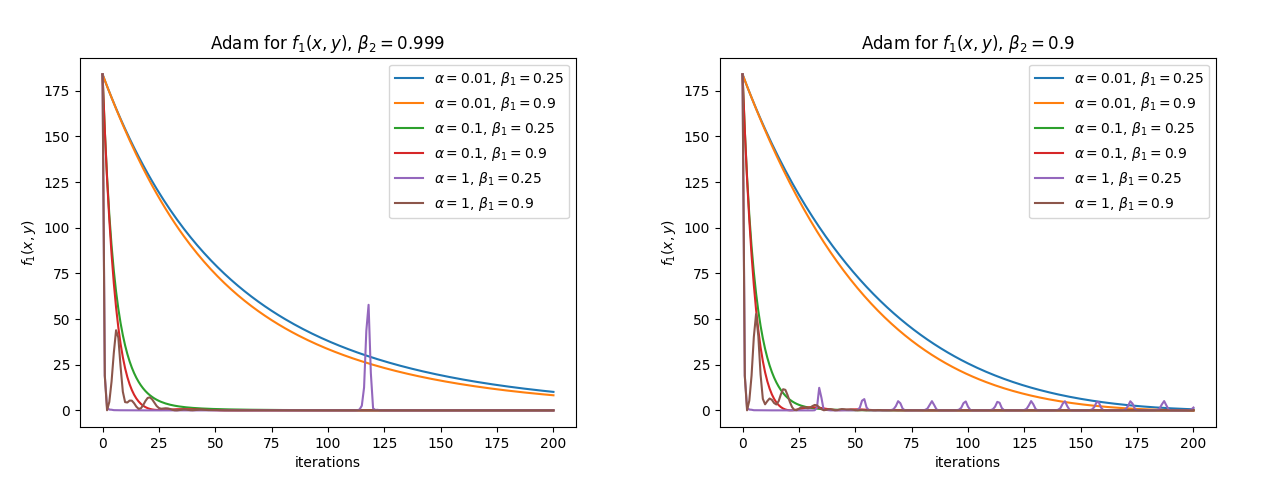
\includegraphics[scale=1.6]{figs/b/b_iii_1.png}
\end{center}

The aforementioned divergences are due to oscillations in the step size of the $y$ parameter seen below (the step sizes for $x$ quickly stabilise and are not plotted here):

\begin{center}
    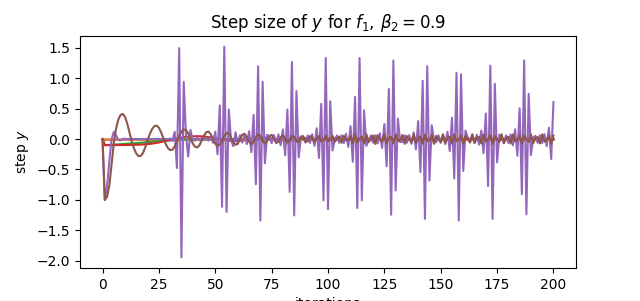
\includegraphics[scale=0.6]{figs/b/b_iii_stepy_f1.png}
\end{center}

For $f_2$ there are no noticeable differences between the results for $\beta_2=0.999$ and $\beta_2=0.9$. In all cases where $\alpha=0.01$ the function does eventually converge on the minimum albeit very slowly and barely within 200 iterations. When $\alpha=1$ the function quickly converges to a point but begins to oscillate around that point indefinitely. When $\alpha=0.1$ and $\beta=0.25$ the function converges on a point quite close to the minimum (0.13) but also begins to oscillate around that point indefinitely. When $\alpha=0.1$ and $\beta=0.9$ the function converges close to the minimum (0.1) but it neither converges completely or begins to oscillate regularly.

\begin{center}
    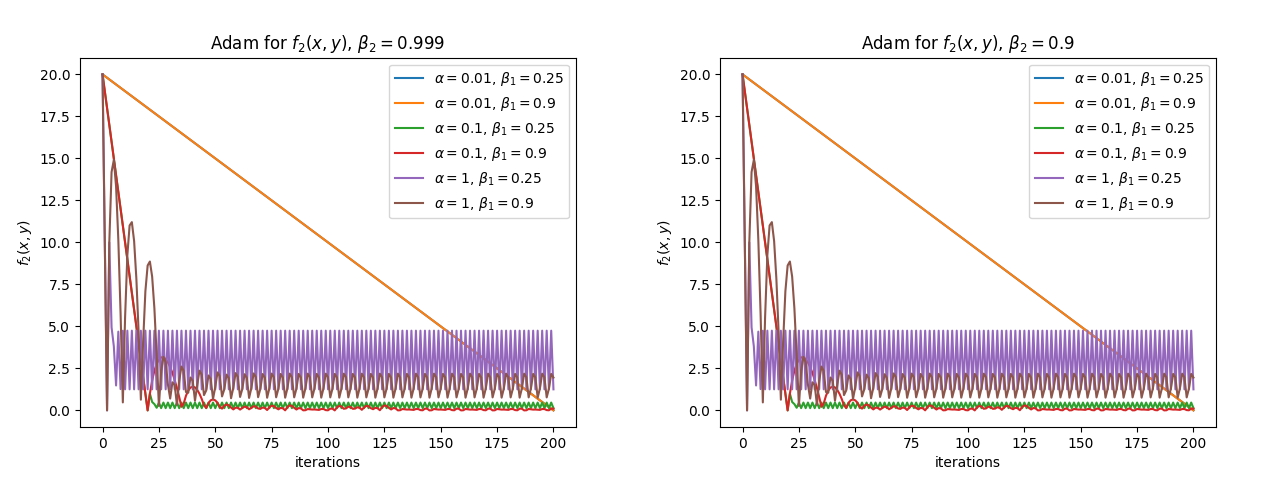
\includegraphics[scale=1.6]{figs/b/b_iii_2.png}
\end{center}

Similarly to $f_1$ the oscillations about a point are due to changes in the step size of $y$ seen below (again, the step sizes for $x$ quickly stabilised):

\begin{center}
    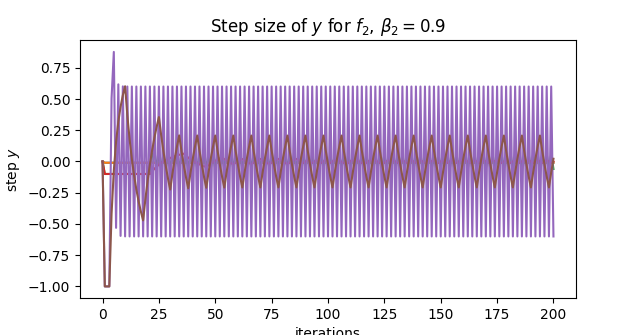
\includegraphics[scale=0.6]{figs/b/b_iii_stepy_f2.png}
\end{center}

In $f_2$ it seems that the cause of the oscillations are due to the gradient of $y$ containing the $sign$ function resulting in it oscillating back and forth about its minimum when the learning rate $\alpha$ is too large.

For $f_1$ the optimal parameters seem to be $\alpha=1$, $\beta_1=0.25$ and $\beta_2=0.999$ although these values could potentially lead to unreliable results due to the odd divergence after around 115 iterations. For $f_2$ no clear optimal parameters present themselves since the only cases that actually converge ($\alpha=0.01$) take almost 200 iterations to do so.

\section*{Question (c)}

Based on the results from question (b) for $f_2$ the following algorithm parameters were chosen: $\alpha_0=0.01, \beta=0.9$ for RMSProp; $\alpha=1, \beta=0.25$ for Heavy Ball; $\alpha=0.01, \beta_1=0.9, \beta_2=0.999$ for Adam. In all cases the algorithms were run for 110 iterations.

\noindent (i) When $x_0=-1$ all of the algorithms converge on the minimum, 0, in a single iteration. The reasons for this are very simple. First of all the value of the function $\max(-1, 0)=0$ is already at its minimum. Secondly given that (1) the value of the gradient $\theta(-1)$ is 0, and (2) all of the algorithms will multiply this gradient by some other calculated value when determining this iteration's step size, we know the resulting step size will be 0 meaning that the function will remain at its minimum indefinitely.

\begin{center}
    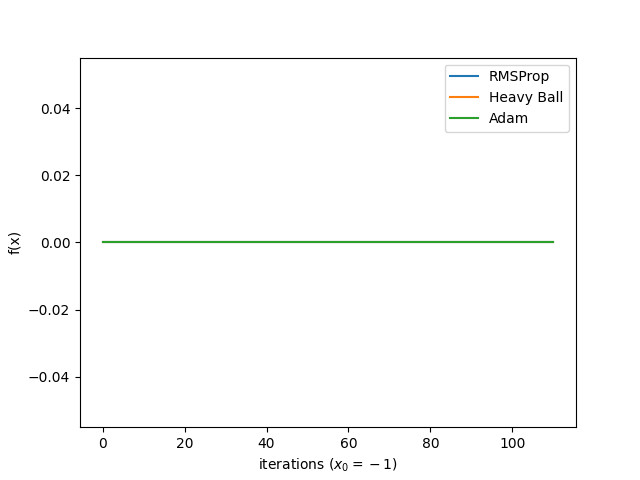
\includegraphics[scale=0.6]{figs/c/c_i.png}
\end{center}

\noindent (ii) When $x_0=+1$ all of the algorithms eventually converge on the minimum. Heavy Ball does so in 2 iterations, RMSProp does so in 91 iterations and Adam does so in 101 iterations.

For Heavy Ball the value of $z$ during the first iteration evaluates to $\frac{1}{1+\epsilon}$. This value is then multiplied by the gradient, $\theta(1)=1$, and decremented from $x_0$. Due to the tiny effect that $\epsilon$ has on the equation the new value of $x$ is slightly larger than the minimum and so requires an additional iteration to converge. If not for the inclusion of $\epsilon$ the algorithm would converge after a single iteration.

For both RMSProp and Adam the functions decrease at an almost constant rate due to the fact that the gradient, $\theta(x)$, remains constant when $x > 0$. For RMSProp there is an slightly faster decrease at the beginning due to $x$ being decremented by the constant $\alpha_0$ initially before the calculated $\alpha$ values take over.

\begin{center}
    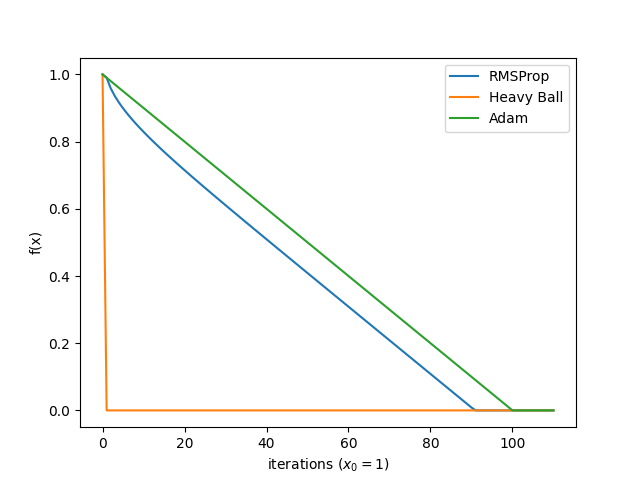
\includegraphics[scale=0.6]{figs/c/c_ii.png}
\end{center}

\noindent (iii) When $x_0=+100$ only the Heavy Ball algorithm converges on the minimum, doing so in 2 iterations. The reason for the Heavy Ball algorithms convergence is exactly the same as when $x_0$ was $+1$: the first iteration decrements $x$ by $\frac{100}{1+\epsilon}$ which is almost enough to reach the minimum (due to $\epsilon$) while the second iteration finishes the job.

\begin{center}
    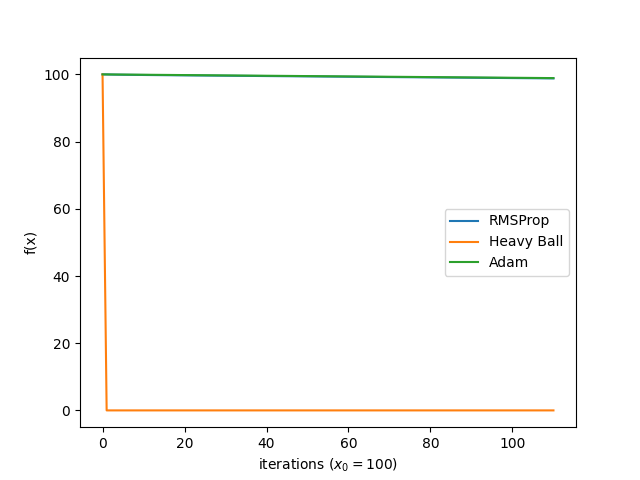
\includegraphics[scale=0.6]{figs/c/c_iii.png}
\end{center}

For RMSProp and Adam the change in the initial value of $x$ has no effect on the rate at which the functions decrease due to value of $f(x)$ never being present in the step size calculation. Only the gradient has any effect on the rate of convergence and, as previously mentioned, it remains constant for $x > 0$. Given that both algorithms converge at same rate as in (ii) they would be expected to converge about 100 times slower, ie after 10000 iterations:

\begin{center}
    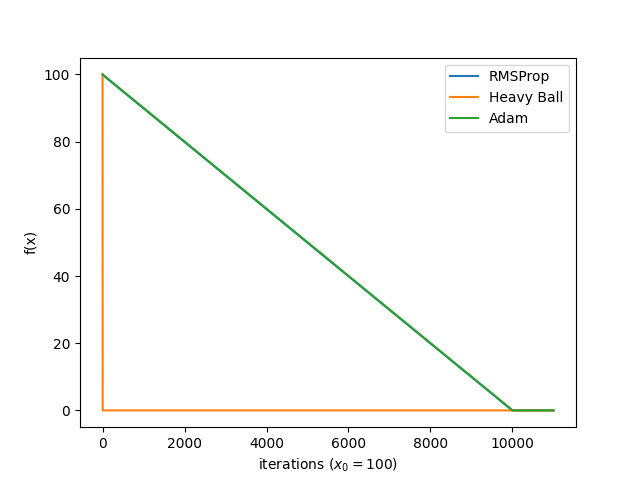
\includegraphics[scale=0.6]{figs/c/c_iii_10k.png}
\end{center}

\section*{Appendix A: Code}

\lstset{basicstyle=\footnotesize,xleftmargin=0in}
\begin{lstlisting}[language=Python]
from copy import deepcopy
import matplotlib.pyplot as plt
import numpy as np
import sympy as sp

def plot_contour(f, x_rng, y_rng, data):
    plt.figure(2)
    X = np.linspace(x_rng[0], x_rng[1], 100)
    Y = np.linspace(y_rng[0], y_rng[1], 100)
    Z = []
    for x in X:
        z = []
        for y in Y: z.append(f(x, y))
        Z.append(z)
    Z = np.array(Z)
    X, Y = np.meshgrid(X, Y)
    plt.contour(X, Y, Z, 10)
    for datum in data:
        Xs = np.array(datum[0])
        Ys = np.array(datum[1])
        plt.plot(Xs, Ys)
        #plt.scatter(Xs[::20], Ys[::20])
    plt.xlim(x_rng)
    plt.ylim(y_rng)
    plt.xlabel('$x$')
    plt.ylabel('$y$')
    plt.show()

def get_function_derivatives():
    x, y = sp.symbols('x y', real=True)
    # function 1
    f1 = (9 * ((x - 5) ** 4)) + (10 * ((y - 2) ** 2))
    df1_x = sp.diff(f1, x)
    df1_y = sp.diff(f1, y)
    print(f1)
    print(df1_x)
    print(df1_y)
    # function 2
    f2 = sp.Max(x - 5, 0) + (10 * sp.Abs(y - 2))
    df2_x = sp.diff(f2, x)
    df2_y = sp.diff(f2, y)
    print(f2)
    print(df2_x)
    print(df2_y)

def gd_polyak(f, df, x0, num_iters=100):
    # boilerplate
    x = deepcopy(x0)
    n = len(df)
    xs, fs, steps = [deepcopy(x)], [f(*x)], []
    # constant parameters
    epsilon = 1e-8
    # iterations
    for _ in range(num_iters):
        # calculate step then update values
        step = f(*x) / (sum(df[i](x[i]) ** 2 for i in range(n)) + epsilon)
        for i in range(n):
            x[i] -= step * df[i](x[i])
        # boilerplate
        xs.append(deepcopy(x))
        fs.append(f(*x))
        steps.append(step)
    return xs, fs, steps

def gd_rms_prop(f, df, x0, params, num_iters=100):
    # boilerplate
    alpha0, beta = params
    x = deepcopy(x0)
    n = len(df)
    xs, fs, steps = [deepcopy(x)], [f(*x)], [[alpha0] * n]
    # constant parameters
    epsilon = 1e-8
    # variable parameters
    sums = [0] * n
    alphas = [alpha0] * n
    # iterations
    for _ in range(num_iters):
        # update values and calculate steps
        for i in range(n):
            x[i] -= alphas[i] * df[i](x[i])
            sums[i] = (beta * sums[i]) + ((1 - beta) * (df[i](x[i]) ** 2))
            alphas[i] = alpha0 / ((sums[i] ** 0.5) + epsilon)
        # boilerplate
        xs.append(deepcopy(x))
        fs.append(f(*x))
        steps.append(deepcopy(alphas))
    return xs, fs, steps

def gd_heavy_ball(f, df, x0, params, num_iters=100):
    # boilerplate
    alpha, beta = params
    x = deepcopy(x0)
    n = len(df)
    xs, fs, steps = [deepcopy(x)], [f(*x)], [0]
    # constant parameters
    epsilon = 1e-8
    # variable parameters
    z = 0
    # iterations
    for _ in range(num_iters):
        # calculate step then update values
        z = (beta * z) + (alpha * f(*x) / (sum(df[i](x[i]) ** 2 for i in range(n)) + epsilon))
        for i in range(n):
            x[i] -= z * df[i](x[i])
        # boilerplate
        xs.append(deepcopy(x))
        fs.append(f(*x))
        steps.append(z)
    return xs, fs, steps

def gd_adam(f, df, x0, params, num_iters=100):
    # boilerplate
    alpha, beta1, beta2 = params
    x = deepcopy(x0)
    n = len(df)
    xs, fs, steps = [deepcopy(x)], [f(*x)], [[0] * n]
    # constant parameters
    epsilon = 1e-8
    # variable parameters
    ms = [0] * n
    vs = [0] * n
    step = [0] * n
    t = 0
    # iterations
    for _ in range(num_iters):
        # calculate steps then update values
        t += 1
        for i in range(n):
            ms[i] = (beta1 * ms[i]) + ((1 - beta1) * df[i](x[i]))
            vs[i] = (beta2 * vs[i]) + ((1 - beta2) * (df[i](x[i]) ** 2))
            m_hat = ms[i] / (1 - (beta1 ** t))
            v_hat = vs[i] / (1 - (beta2 ** t))
            step[i] = alpha * (m_hat / ((v_hat ** 0.5) + epsilon))
            x[i] -= step[i]
        # boilerplate
        xs.append(deepcopy(x))
        fs.append(f(*x))
        steps.append(deepcopy(step))
    return xs, fs, steps

def part_b_i(f, df, x, fnum):
    alpha0s = [0.001, 0.01, 0.1]
    betas = [0.25, 0.9]
    num_iters = 200
    iters = list(range(num_iters + 1))
    legend = []
    for alpha0 in alpha0s:
        for beta in betas:
            xs, values, steps = gd_rms_prop(f, df, x, [alpha0, beta], num_iters=num_iters)
            print(f'alpha0={alpha0}, beta={beta}: final_value={values[-1]}')
            plt.figure(1)
            plt.plot(iters, values)
            stepsx = [step[0] for step in steps]
            stepsy = [step[1] for step in steps]
            plt.figure(2)
            plt.plot(iters, stepsx)
            plt.figure(3)
            plt.plot(iters, stepsy)
    plt.figure(1)
    plt.xlabel('iterations')
    plt.ylabel(f'$f_{fnum}(x,y)$')
    plt.title(f'RMSProp for $f_{fnum}(x,y)$')
    if fnum == 1: plt.ylim([0, 100])
    plt.legend(legend)
    plt.figure(2)
    plt.xlabel('iterations')
    plt.ylabel('step $x$')
    plt.title(f'Step size of $x$ for $f_{fnum}$')
    plt.figure(3)
    plt.xlabel('iterations')
    plt.ylabel('step $y$')
    plt.title(f'Step size of $y$ for $f_{fnum}$')
    plt.show()
    
def part_b_ii(f, df, x, fnum):
    alphas = [0.01, 0.1, 1]
    betas = [0.25, 0.9]
    num_iters = 200
    iters = list(range(num_iters + 1))
    legend = []
    contour_data = []
    for alpha in alphas:
        for beta in betas:
            xs, values, steps = gd_heavy_ball(f, df, x, [alpha, beta], num_iters=num_iters)
            legend.append(f'$\\alpha={alpha},\\, \\beta={beta}$')
            print(f'alpha={alpha}, beta={beta}: final_value={values[-1]}')
            plt.plot(iters, values)
    plt.xlabel('iterations')
    plt.ylabel(f'$f_{fnum}(x,y)$')
    plt.title(f'Heavy Ball for $f_{fnum}(x,y)$')
    if fnum == 1: plt.ylim([0, 200])
    else: plt.ylim([0, 30])
    plt.legend(legend)
    plt.show()

def part_b_iii(f, df, x, fnum):
    alphas = [0.01, 0.1, 1]
    beta1s = [0.25, 0.9]
    beta2s = [0.9, 0.999]
    num_iters = 200
    iters = list(range(num_iters + 1))
    legend = []
    for beta2 in beta2s:
        for alpha in alphas:
            for beta1 in beta1s:
                xs, values, steps = gd_adam(f, df, x, [alpha, beta1, beta2], num_iters=num_iters)
                legend.append(f'$\\alpha={alpha},\\, \\beta_1={beta1}$')
                print(f'alpha={alpha}, beta1={beta1}, beta2={beta2}: final_value={values[-1]}')
                plt.figure(1)
                plt.plot(iters, values)
                stepsx = [step[0] for step in steps]
                stepsy = [step[1] for step in steps]
                plt.figure(2)
                plt.plot(iters, stepsx)
                plt.figure(3)
                plt.plot(iters, stepsy)
        plt.figure(1)
        plt.xlabel('iterations')
        plt.ylabel(f'$f_{fnum}(x,y)$')
        plt.title(f'Adam for $f_{fnum}(x,y),\\, \\beta_2={beta2}$')
        plt.legend(legend)
        plt.figure(2)
        plt.xlabel('iterations')
        plt.ylabel('step $x$')
        plt.title(f'Step size of $x$ for $f_{fnum},\\, \\beta_2={beta2}$')
        plt.figure(3)
        plt.xlabel('iterations')
        plt.ylabel('step $y$')
        plt.title(f'Step size of $y$ for $f_{fnum},\\, \\beta_2={beta2}$')
        plt.show()

def part_b():
    f1 = lambda x, y: 9*(x - 5)**4 + 10*(y - 2)**2
    df1_x = lambda x: 36*(x - 5)**3
    df1_y = lambda y: 20*y - 40
    f2 = lambda x, y: 10*abs(y - 2) + max(0, x - 5)
    df2_x = lambda x: np.heaviside(x - 5, 0)
    df2_y = lambda y: 10*np.sign(y - 2)
    print('(b)(i) f1')
    part_b_i(f1, [df1_x, df1_y], [3, 0], 1)
    print('(b)(i) f2')
    part_b_i(f2, [df2_x, df2_y], [3, 0], 2)
    print('(b)(ii) f1')
    part_b_ii(f1, [df1_x, df1_y], [3, 0], 1)
    print('(b)(ii) f2')
    part_b_ii(f2, [df2_x, df2_y], [3, 0], 2)
    print('(b)(iii) f1')
    part_b_iii(f1, [df1_x, df1_y], [3, 0], 1)
    print('(b)(iii) f2')
    part_b_iii(f2, [df2_x, df2_y], [3, 0], 2)

def part_c():
    f = lambda x: max(x, 0)
    df = lambda x: np.heaviside(x, 0)
    num_iters = 110
    iters = list(range(num_iters + 1))
    # parts (i), (ii) and (iii)
    for x0 in [-1, 1, 100]:
        _, values, _ = gd_rms_prop(f, [df], [x0], [0.01, 0.9], num_iters=num_iters)
        #print(x0, values)
        print(f'RMSProp (x0={x0}): {values[-1]}')
        plt.plot(iters, values)
        _, values, _ = gd_heavy_ball(f, [df], [x0], [1, 0.25], num_iters=num_iters)
        #print(x0, values)
        print(f'Heavy Ball (x0={x0}): {values[-1]}')
        plt.plot(iters, values)
        _, values, _ = gd_adam(f, [df], [x0], [0.01, 0.9, 0.999], num_iters=num_iters)
        #print(x0, values)
        print(f'Adam (x0={x0}): {values[-1]}')
        plt.plot(iters, values)
        plt.xlabel(f'iterations ($x_0={x0}$)')
        plt.ylabel('f(x)')
        plt.legend(['RMSProp', 'Heavy Ball', 'Adam'])
        plt.show()

#get_function_derivatives()
part_b()
#part_c()
\end{lstlisting}

\end{document}
